\def\year{2015}
\documentclass[letterpaper]{article}
\usepackage{aaai}
\usepackage{fixbib}
\usepackage{times}
\usepackage{helvet}
\usepackage{courier}
%\usepackage[dvipdfmx]{graphicx}
\usepackage{graphicx}
\usepackage{amsmath}
\usepackage{amsfonts}
\usepackage{url}
\frenchspacing
\setlength{\pdfpagewidth}{8.5in}
\setlength{\pdfpageheight}{11in}
\pdfinfo{
/Title (Insert Your Title Here)
/Author (Put All Your Authors Here, Separated by Commas)}
\begin{document}
%
\title{Bayesian Optimization for Shortest Path Prediction}
\author{CS4246 Project: Planning and Decision Making in the Real World  \\ \\
{\bf Team 04} \\
Huang Wei Ling, A0101200R\\
Nathan Azaria, A0113011L\\
Ng Hui Xian Lynnette, A0119646X\\
Nguyen Duc Thien, A0093587M\\
Oh Shunhao, A0065475X\\
}
\maketitle
\begin{abstract}
\begin{quote}
Computing shortest paths is relevant to tackle issues in events such as resource management. Event space is usually limited and there are many concurrent activities at any point of time. Therefore, the computation of shortest paths allow the event committee to plan the layout and schedule of the programs in an event effectively and allows participants of the event to move around the event space efficiently so that they gain most out of attending the event. \\

In this report, we illustrate the use of Bayesian Optimization to find a set of reference points at significant points in an area. For each data point, we compute the shortest paths from the data point to each of the reference points.
\end{quote}
\end{abstract}

\section{Introduction}
In this report, we propose the use of Bayesian Optimization for computation of shortest paths. Particularly, we discuss how we exploit the properties of Bayesian Optimization to find a set of reference points at significant points in an area for path prediction, the critical requirements of our proposed application as well as how people can make use of the results of our analysis to plan and make decisions for future crowd controlling or crowd management. \\

We also touch on the technical details which includes how the different components of the . We also outline the experimental plan we use to perform and evaluate the performance of Gaussian Processes for modelling of crowds. \\

The rationale behind using Gaussian Processes for modelling of crowds is to do better crowd control by predicting the population density within any defined region. For example, it can be useful in the case of train breakdowns to facilitate crowd movements. In addition, we can perform path prediction using the GP model.

\section{Motivating Application}



\subsection{The use of Bayesian Optimization}

Minimise $f(x)$

In our case, $x$ refers to the input points $c1, c2, c3$

\subsection{Qualitative Advantages}



\subsection{Important Requirements}



\section{Technical Approach}



\subsection{Shortest Path}

We note that in the original data, the positions of each individual at any point of time is given in Cartesian coordinates $(x,y)$. The first step is thus to convert the existing Cartesian coordinates of each person's location specified in the data into a 3-tuple of shortest-path coordinates, $s_1, s_2, s_3$, referring to the shortest paths from the current position to each of the three reference points respectively.\\

\begin{figure}[!h]
  \centering
    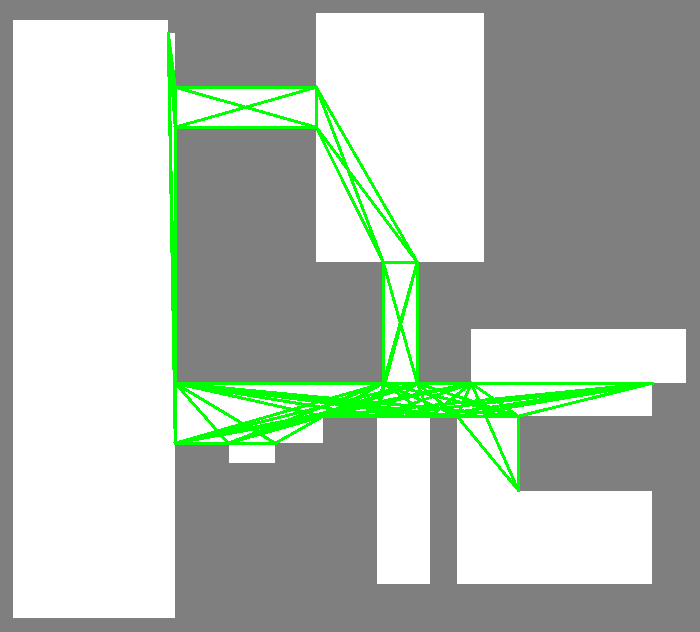
\includegraphics[width=170px]{diagrams/floor18visibilitygraph.png}
  \caption{Visibility Graph generated over the 18th floor of the XXXX building}
  \label{fig:floor18vg}
\end{figure}

Shortest path coordinates are computed using Any-Angle Pathfinding algorithms on grids. A floorplan of the area is used, and abstracted into a grid of blocked and unblocked tiles, representing impassable and passable areas in the actual space respectively. Then, for each $(x,y)$ coordinate in the data, we map it to the nearest unblocked tile on the grid. This can be done efficiently using Kd-trees.\\

\begin{figure}[!h]
  \centering
    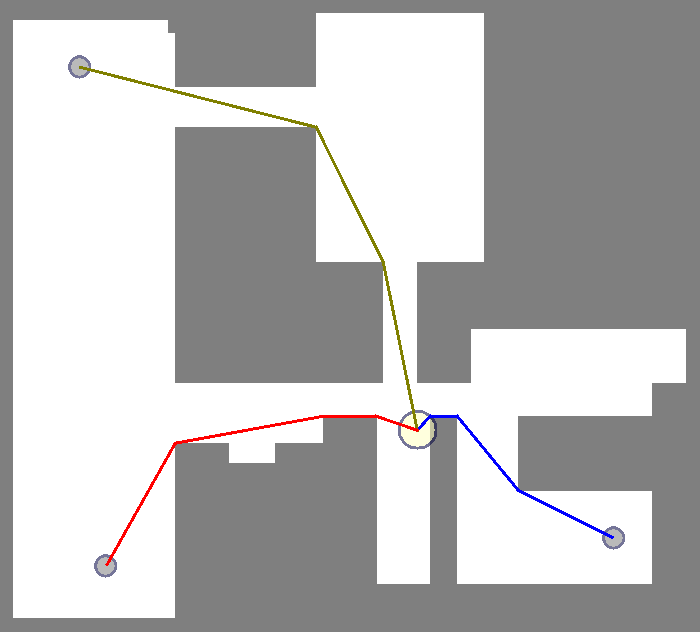
\includegraphics[width=170px]{diagrams/floor18shortestpaths.png}
  \caption{Shortest any-angle paths computed from a single point to three different reference points.}
  \label{fig:floor18sps}
\end{figure}

We then apply an optimal any-angle pathfinding algorithm to compute the shortest path from the $(x,y)$ coordinate to each of the three reference points. This generates three shortest-path queries for each user position. This shortest path computation can be done efficiently as a batch, on an approximately 100x100 grid by preprocessing a visibility graph like shown on Figure \ref{fig:floor18vg}, which can be reused to process each of the shortest path queries (Figure \ref{fig:floor18sps}). Running the A* algorithm on visibility graphs is an optimal offline algorithm for Any-Angle Pathfinding.\footnote{Visibility graph algorithm \url{https://github.com/Ohohcakester/Any-Angle-Pathfinding}}\\

Thus for each point, as there are three reference points, we obtain three shortest-path coordinates, $s_1, s_2, s_3$.\\

\subsection{Gaussian Process}

Instead of applying the Gaussian Processes to the Cartesian coordinates as before, we apply it to the shortest-path coordinates, $s_1, s_2, s_3$, over time.

Similar to before, the shortest path coordinates are modelled as a time series, and each of the three coordinates are regressed independently over time using the Gaussian Process model.

The hope is that with a good selection of reference points, the coordinates $s_1, s_2, s_3$ can be regarded as independent of each other without a significant loss of accuracy.

From the regression, we obtain, at each point of time, a probability distribution of each of the coordinates $s_1, s_2, s_3$, described as a joint a normal distribution $\mathcal{N}\tilde (\boldsymbol{\mu},\sigma^2)$.

\subsection{Density Computation}

The use of shortest-path coordinates over Cartesian coordinates makes density computation more challenging. We can no longer simply select an arbitrary region (e.g. a rectangle) and integrate the probability distribution over all $x$ and $y$ values that fall within the region. We cannot even assume a one-to-one mapping between the shortest-path coordinates and the Cartesian coordinates.

Thus the integration has to be carried out differently. Instead of picking a rectangle in the Cartesian plane, we integrate over rectangles defined over the shortest-path coordinates. A rectangle is defined as the set $\{(s_1,s_2,s_3) : a_1\leq s_1\leq b_1, a_2\leq s_2\leq b_2, a_3\leq s_3\leq b_3\}$ for some $a_1,b_1,a_2,b_2,a_3,b_3 \in \mathbb{R}$.

To do this, we first note that for each shortest-path coordinate $s_i$, $s_i$ lies within some bounded interval $[0,D_i]$, for some $D_i > 0$.



\subsection{Error Computation}


\subsection{Additional Insights}


\subsection{Improvement}



\section{Experimental Evaluation}



\subsection{Real-World Dataset}



\subsection{Experimental Setup}



\section{Conclusion}



\section{6. Main Roles of Each Member}
\begin{itemize}
\item \textbf{Wei Ling}: 
Writing of the report, keeping track of requirements, and research.
\item \textbf{Nathan}: 
Setting up of the experiment and running the tests using the dataset.
\item \textbf{Lynnette}: 
Setting up and experimenting with the various libraries and available tools, and fine-tuning the Gaussian Process models
\item \textbf{Thien}: 
Setting up and experimenting with the various libraries and available tools, and fine-tuning the Gaussian Process models
\item \textbf{Shunhao}: 
Problem formulation and modelling, mathematics, creating the visualisations and experiment, and writing the report.
\end{itemize}

\bibliographystyle{aaai}
\bibliography{report}

\end{document}
